\documentclass{scrartcl}
\usepackage{mathtools}
\usepackage{tikz}
\usetikzlibrary{trees,positioning}

\begin{document}
\begin{figure}
\centering
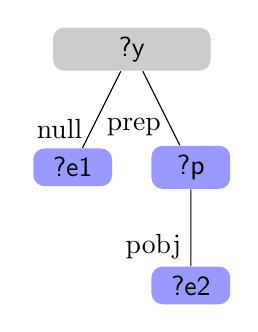
\begin{tikzpicture}
\node[fill = gray!40, shape = rectangle, rounded corners, minimum width = 2cm, font = \sffamily] (0) {?y}
child {node[fill = blue!40, shape = rectangle, rounded corners, minimum width = 1cm, font = \sffamily]  (1) {?e1}
}
child {node[fill = blue!40, shape = rectangle, rounded corners, minimum width = 1cm, font = \sffamily]  (2) {?p}
child {node[fill = blue!40, shape = rectangle, rounded corners, minimum width = 1cm, font = \sffamily] (3) {?e2}
}
};
\begin{scope}[nodes = {draw = none}]
\path (1)     -- (0) node [near start, left]  {\text{null}};
\path (2)     -- (0) node [near start, left]  {\text{prep}};
\path (3)     -- (2) node [near start, left]  {\text{pobj}};
\draw[densely dashed, rounded corners, thin];
\end{scope} 
\end{tikzpicture}
\caption{Visualisation for SPARQLPattern\_EN\_1}
\label{fig:SPARQLPatternEN1}
\end{figure}


\begin{figure}
\centering
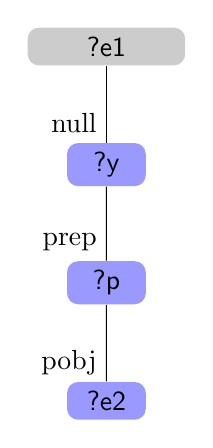
\begin{tikzpicture}
\node[fill = gray!40, shape = rectangle, rounded corners, minimum width = 2cm, font = \sffamily] (3) {?e1}
child {node[fill = blue!40, shape = rectangle, rounded corners, minimum width = 1cm, font = \sffamily]  (4) {?y}
child {node[fill = blue!40, shape = rectangle, rounded corners, minimum width = 1cm, font = \sffamily] (5) {?p}
child {node[fill = blue!40, shape = rectangle, rounded corners, minimum width = 1cm, font = \sffamily] (6) {?e2}
}
}};
\begin{scope}[nodes = {draw = none}]
\path (4)     -- (3) node [near start, left]  {\text{null}};
\path (5)     -- (4) node [near start, left]  {\text{prep}};
\path (6)     -- (5) node [near start, left]  {\text{pobj}};
\draw[densely dashed, rounded corners, thin];
\end{scope} 
\end{tikzpicture}
\caption{Visualisation for SPARQLPattern\_EN\_2}
\label{fig:SPARQLPatternEN2}
\end{figure}


\begin{figure}
\centering
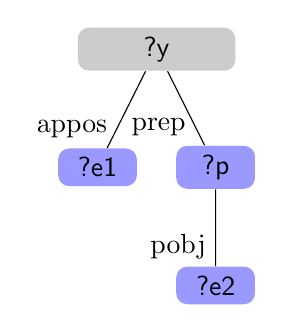
\begin{tikzpicture}
\node[fill = gray!40, shape = rectangle, rounded corners, minimum width = 2cm, font = \sffamily] (6) {?y}
child {node[fill = blue!40, shape = rectangle, rounded corners, minimum width = 1cm, font = \sffamily]  (7) {?e1}
}
child {node[fill = blue!40, shape = rectangle, rounded corners, minimum width = 1cm, font = \sffamily]  (8) {?p}
child {node[fill = blue!40, shape = rectangle, rounded corners, minimum width = 1cm, font = \sffamily] (9) {?e2}
}
};
\begin{scope}[nodes = {draw = none}]
\path (7)     -- (6) node [near start, left]  {\text{appos}};
\path (8)     -- (6) node [near start, left]  {\text{prep}};
\path (9)     -- (8) node [near start, left]  {\text{pobj}};
\draw[densely dashed, rounded corners, thin];
\end{scope} 
\end{tikzpicture}
\caption{Visualisation for SPARQLPattern\_EN\_3}
\label{fig:SPARQLPatternEN3}
\end{figure}


\begin{figure}
\centering
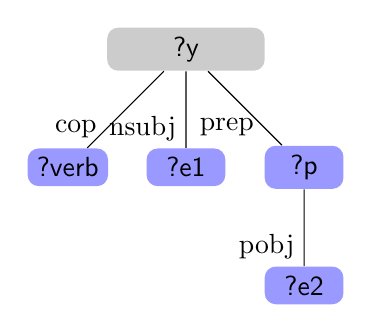
\begin{tikzpicture}
\node[fill = gray!40, shape = rectangle, rounded corners, minimum width = 2cm, font = \sffamily] (9) {?y}
child {node[fill = blue!40, shape = rectangle, rounded corners, minimum width = 1cm, font = \sffamily]  (10) {?verb}
}
child {node[fill = blue!40, shape = rectangle, rounded corners, minimum width = 1cm, font = \sffamily]  (11) {?e1}
}
child {node[fill = blue!40, shape = rectangle, rounded corners, minimum width = 1cm, font = \sffamily]  (12) {?p}
child {node[fill = blue!40, shape = rectangle, rounded corners, minimum width = 1cm, font = \sffamily] (13) {?e2}
}
};
\begin{scope}[nodes = {draw = none}]
\path (10)     -- (9) node [near start, left]  {\text{cop}};
\path (11)     -- (9) node [near start, left]  {\text{nsubj}};
\path (12)     -- (9) node [near start, left]  {\text{prep}};
\path (13)     -- (12) node [near start, left]  {\text{pobj}};
\draw[densely dashed, rounded corners, thin];
\end{scope} 
\end{tikzpicture}
\caption{Visualisation for SPARQLPattern\_EN\_4}
\label{fig:SPARQLPatternEN4}
\end{figure}


\begin{figure}
\centering
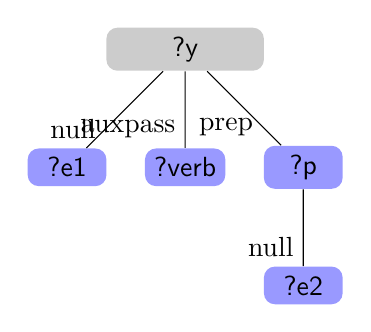
\begin{tikzpicture}
\node[fill = gray!40, shape = rectangle, rounded corners, minimum width = 2cm, font = \sffamily] (13) {?y}
child {node[fill = blue!40, shape = rectangle, rounded corners, minimum width = 1cm, font = \sffamily]  (14) {?e1}
}
child {node[fill = blue!40, shape = rectangle, rounded corners, minimum width = 1cm, font = \sffamily]  (15) {?verb}
}
child {node[fill = blue!40, shape = rectangle, rounded corners, minimum width = 1cm, font = \sffamily]  (16) {?p}
child {node[fill = blue!40, shape = rectangle, rounded corners, minimum width = 1cm, font = \sffamily] (17) {?e2}
}
};
\begin{scope}[nodes = {draw = none}]
\path (14)     -- (13) node [near start, left]  {\text{null}};
\path (15)     -- (13) node [near start, left]  {\text{auxpass}};
\path (16)     -- (13) node [near start, left]  {\text{prep}};
\path (17)     -- (16) node [near start, left]  {\text{null}};
\draw[densely dashed, rounded corners, thin];
\end{scope} 
\end{tikzpicture}
\caption{Visualisation for SPARQLPattern\_EN\_5}
\label{fig:SPARQLPatternEN5}
\end{figure}


\begin{figure}
\centering
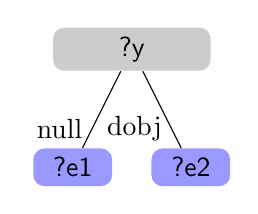
\begin{tikzpicture}
\node[fill = gray!40, shape = rectangle, rounded corners, minimum width = 2cm, font = \sffamily] (17) {?y}
child {node[fill = blue!40, shape = rectangle, rounded corners, minimum width = 1cm, font = \sffamily]  (18) {?e1}
}
child {node[fill = blue!40, shape = rectangle, rounded corners, minimum width = 1cm, font = \sffamily]  (19) {?e2}
}
;
\begin{scope}[nodes = {draw = none}]
\path (18)     -- (17) node [near start, left]  {\text{null}};
\path (19)     -- (17) node [near start, left]  {\text{dobj}};
\draw[densely dashed, rounded corners, thin];
\end{scope} 
\end{tikzpicture}
\caption{Visualisation for SPARQLPattern\_EN\_6}
\label{fig:SPARQLPatternEN6}
\end{figure}


\begin{figure}
\centering
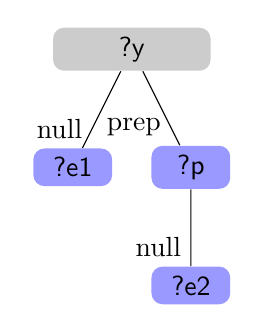
\begin{tikzpicture}
\node[fill = gray!40, shape = rectangle, rounded corners, minimum width = 2cm, font = \sffamily] (19) {?y}
child {node[fill = blue!40, shape = rectangle, rounded corners, minimum width = 1cm, font = \sffamily]  (20) {?e1}
}
child {node[fill = blue!40, shape = rectangle, rounded corners, minimum width = 1cm, font = \sffamily]  (21) {?p}
child {node[fill = blue!40, shape = rectangle, rounded corners, minimum width = 1cm, font = \sffamily] (22) {?e2}
}
};
\begin{scope}[nodes = {draw = none}]
\path (20)     -- (19) node [near start, left]  {\text{null}};
\path (21)     -- (19) node [near start, left]  {\text{prep}};
\path (22)     -- (21) node [near start, left]  {\text{null}};
\draw[densely dashed, rounded corners, thin];
\end{scope} 
\end{tikzpicture}
\caption{Visualisation for SPARQLPattern\_EN\_7}
\label{fig:SPARQLPatternEN7}
\end{figure}


\begin{figure}
\centering
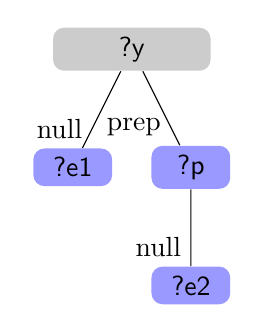
\begin{tikzpicture}
\node[fill = gray!40, shape = rectangle, rounded corners, minimum width = 2cm, font = \sffamily] (22) {?y}
child {node[fill = blue!40, shape = rectangle, rounded corners, minimum width = 1cm, font = \sffamily]  (23) {?e1}
}
child {node[fill = blue!40, shape = rectangle, rounded corners, minimum width = 1cm, font = \sffamily]  (24) {?p}
child {node[fill = blue!40, shape = rectangle, rounded corners, minimum width = 1cm, font = \sffamily] (25) {?e2}
}
};
\begin{scope}[nodes = {draw = none}]
\path (23)     -- (22) node [near start, left]  {\text{null}};
\path (24)     -- (22) node [near start, left]  {\text{prep}};
\path (25)     -- (24) node [near start, left]  {\text{null}};
\draw[densely dashed, rounded corners, thin];
\end{scope} 
\end{tikzpicture}
\caption{Visualisation for SPARQLPattern\_EN\_8}
\label{fig:SPARQLPatternEN8}
\end{figure}


\begin{figure}
\centering
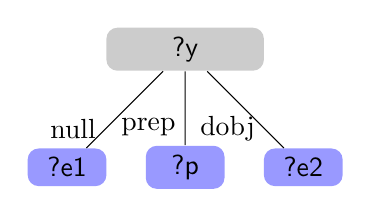
\begin{tikzpicture}
\node[fill = gray!40, shape = rectangle, rounded corners, minimum width = 2cm, font = \sffamily] (25) {?y}
child {node[fill = blue!40, shape = rectangle, rounded corners, minimum width = 1cm, font = \sffamily]  (26) {?e1}
}
child {node[fill = blue!40, shape = rectangle, rounded corners, minimum width = 1cm, font = \sffamily]  (27) {?p}
}
child {node[fill = blue!40, shape = rectangle, rounded corners, minimum width = 1cm, font = \sffamily]  (28) {?e2}
}
;
\begin{scope}[nodes = {draw = none}]
\path (26)     -- (25) node [near start, left]  {\text{null}};
\path (27)     -- (25) node [near start, left]  {\text{prep}};
\path (28)     -- (25) node [near start, left]  {\text{dobj}};
\draw[densely dashed, rounded corners, thin];
\end{scope} 
\end{tikzpicture}
\caption{Visualisation for SPARQLPattern\_EN\_1}
\label{fig:SPARQLPatternEN1}
\end{figure}


\begin{figure}
\centering
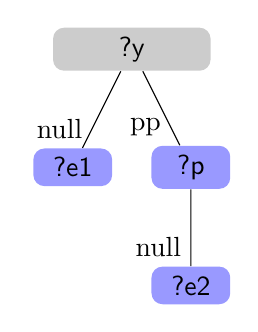
\begin{tikzpicture}
\node[fill = gray!40, shape = rectangle, rounded corners, minimum width = 2cm, font = \sffamily] (28) {?y}
child {node[fill = blue!40, shape = rectangle, rounded corners, minimum width = 1cm, font = \sffamily]  (29) {?e1}
}
child {node[fill = blue!40, shape = rectangle, rounded corners, minimum width = 1cm, font = \sffamily]  (30) {?p}
child {node[fill = blue!40, shape = rectangle, rounded corners, minimum width = 1cm, font = \sffamily] (31) {?e2}
}
};
\begin{scope}[nodes = {draw = none}]
\path (29)     -- (28) node [near start, left]  {\text{null}};
\path (30)     -- (28) node [near start, left]  {\text{pp}};
\path (31)     -- (30) node [near start, left]  {\text{null}};
\draw[densely dashed, rounded corners, thin];
\end{scope} 
\end{tikzpicture}
\caption{Visualisation for SPARQLPattern\_DE\_1}
\label{fig:SPARQLPatternDE1}
\end{figure}


\begin{figure}
\centering
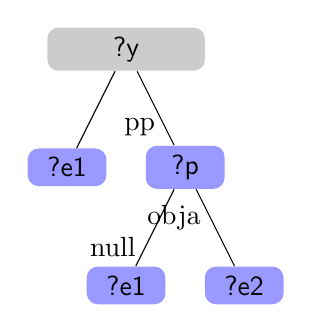
\begin{tikzpicture}
\node[fill = gray!40, shape = rectangle, rounded corners, minimum width = 2cm, font = \sffamily] (31) {?y}
child {node[fill = blue!40, shape = rectangle, rounded corners, minimum width = 1cm, font = \sffamily]  (32) {?e1}
}
child {node[fill = blue!40, shape = rectangle, rounded corners, minimum width = 1cm, font = \sffamily]  (33) {?p}
child {node[fill = blue!40, shape = rectangle, rounded corners, minimum width = 1cm, font = \sffamily] (34) {?e1}
}
child {node[fill = blue!40, shape = rectangle, rounded corners, minimum width = 1cm, font = \sffamily]  (35) {?e2}
}
};
\begin{scope}[nodes = {draw = none}]
\path (34)     -- (33) node [near start, left]  {\text{null}};
\path (33)     -- (31) node [near start, left]  {\text{pp}};
\path (35)     -- (31) node [near start, left]  {\text{obja}};
\draw[densely dashed, rounded corners, thin];
\end{scope} 
\end{tikzpicture}
\caption{Visualisation for SPARQLPattern\_DE\_2}
\label{fig:SPARQLPatternDE2}
\end{figure}


\begin{figure}
\centering
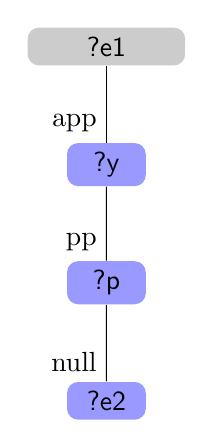
\begin{tikzpicture}
\node[fill = gray!40, shape = rectangle, rounded corners, minimum width = 2cm, font = \sffamily] (35) {?e1}
child {node[fill = blue!40, shape = rectangle, rounded corners, minimum width = 1cm, font = \sffamily]  (36) {?y}
child {node[fill = blue!40, shape = rectangle, rounded corners, minimum width = 1cm, font = \sffamily] (37) {?p}
child {node[fill = blue!40, shape = rectangle, rounded corners, minimum width = 1cm, font = \sffamily] (38) {?e2}
}
}};
\begin{scope}[nodes = {draw = none}]
\path (36)     -- (35) node [near start, left]  {\text{app}};
\path (37)     -- (36) node [near start, left]  {\text{pp}};
\path (38)     -- (37) node [near start, left]  {\text{null}};
\draw[densely dashed, rounded corners, thin];
\end{scope} 
\end{tikzpicture}
\caption{Visualisation for SPARQLPattern\_DE\_3}
\label{fig:SPARQLPatternDE3}
\end{figure}


\begin{figure}
\centering
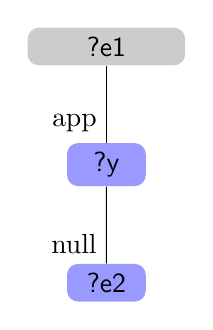
\begin{tikzpicture}
\node[fill = gray!40, shape = rectangle, rounded corners, minimum width = 2cm, font = \sffamily] (38) {?e1}
child {node[fill = blue!40, shape = rectangle, rounded corners, minimum width = 1cm, font = \sffamily]  (39) {?y}
child {node[fill = blue!40, shape = rectangle, rounded corners, minimum width = 1cm, font = \sffamily] (40) {?e2}
}
};
\begin{scope}[nodes = {draw = none}]
\path (39)     -- (38) node [near start, left]  {\text{app}};
\path (40)     -- (39) node [near start, left]  {\text{null}};
\draw[densely dashed, rounded corners, thin];
\end{scope} 
\end{tikzpicture}
\caption{Visualisation for SPARQLPattern\_DE\_4}
\label{fig:SPARQLPatternDE4}
\end{figure}


\begin{figure}
\centering
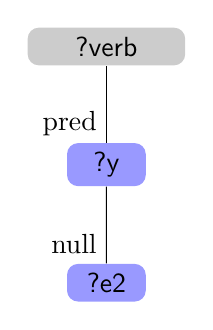
\begin{tikzpicture}
\node[fill = gray!40, shape = rectangle, rounded corners, minimum width = 2cm, font = \sffamily] (40) {?verb}
child {node[fill = blue!40, shape = rectangle, rounded corners, minimum width = 1cm, font = \sffamily]  (41) {?y}
child {node[fill = blue!40, shape = rectangle, rounded corners, minimum width = 1cm, font = \sffamily] (42) {?e2}
}
};
\begin{scope}[nodes = {draw = none}]
\path (41)     -- (40) node [near start, left]  {\text{pred}};
\path (42)     -- (41) node [near start, left]  {\text{null}};
\draw[densely dashed, rounded corners, thin];
\end{scope} 
\end{tikzpicture}
\caption{Visualisation for SPARQLPattern\_DE\_6}
\label{fig:SPARQLPatternDE6}
\end{figure}


\begin{figure}
\centering
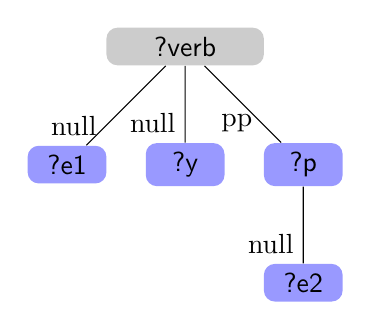
\begin{tikzpicture}
\node[fill = gray!40, shape = rectangle, rounded corners, minimum width = 2cm, font = \sffamily] (42) {?verb}
child {node[fill = blue!40, shape = rectangle, rounded corners, minimum width = 1cm, font = \sffamily]  (43) {?e1}
}
child {node[fill = blue!40, shape = rectangle, rounded corners, minimum width = 1cm, font = \sffamily]  (44) {?y}
}
child {node[fill = blue!40, shape = rectangle, rounded corners, minimum width = 1cm, font = \sffamily]  (45) {?p}
child {node[fill = blue!40, shape = rectangle, rounded corners, minimum width = 1cm, font = \sffamily] (46) {?e2}
}
};
\begin{scope}[nodes = {draw = none}]
\path (43)     -- (42) node [near start, left]  {\text{null}};
\path (44)     -- (42) node [near start, left]  {\text{null}};
\path (45)     -- (42) node [near start, left]  {\text{pp}};
\path (46)     -- (45) node [near start, left]  {\text{null}};
\draw[densely dashed, rounded corners, thin];
\end{scope} 
\end{tikzpicture}
\caption{Visualisation for SPARQLPattern\_DE\_7}
\label{fig:SPARQLPatternDE7}
\end{figure}


\begin{figure}
\centering
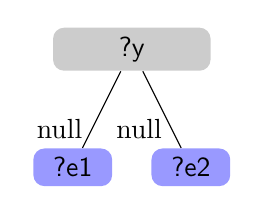
\begin{tikzpicture}
\node[fill = gray!40, shape = rectangle, rounded corners, minimum width = 2cm, font = \sffamily] (46) {?y}
child {node[fill = blue!40, shape = rectangle, rounded corners, minimum width = 1cm, font = \sffamily]  (47) {?e1}
}
child {node[fill = blue!40, shape = rectangle, rounded corners, minimum width = 1cm, font = \sffamily]  (48) {?e2}
}
;
\begin{scope}[nodes = {draw = none}]
\path (47)     -- (46) node [near start, left]  {\text{null}};
\path (48)     -- (46) node [near start, left]  {\text{null}};
\draw[densely dashed, rounded corners, thin];
\end{scope} 
\end{tikzpicture}
\caption{Visualisation for SPARQLPattern\_DE\_8}
\label{fig:SPARQLPatternDE8}
\end{figure}


\begin{figure}
\centering
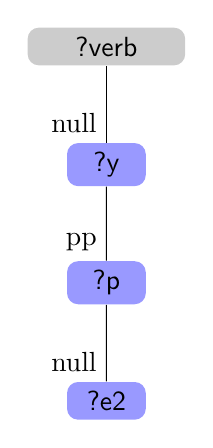
\begin{tikzpicture}
\node[fill = gray!40, shape = rectangle, rounded corners, minimum width = 2cm, font = \sffamily] (48) {?verb}
child {node[fill = blue!40, shape = rectangle, rounded corners, minimum width = 1cm, font = \sffamily]  (49) {?y}
child {node[fill = blue!40, shape = rectangle, rounded corners, minimum width = 1cm, font = \sffamily] (50) {?p}
child {node[fill = blue!40, shape = rectangle, rounded corners, minimum width = 1cm, font = \sffamily] (51) {?e2}
}
}};
\begin{scope}[nodes = {draw = none}]
\path (49)     -- (48) node [near start, left]  {\text{null}};
\path (50)     -- (49) node [near start, left]  {\text{pp}};
\path (51)     -- (50) node [near start, left]  {\text{null}};
\draw[densely dashed, rounded corners, thin];
\end{scope} 
\end{tikzpicture}
\caption{Visualisation for SPARQLPattern\_DE\_9}
\label{fig:SPARQLPatternDE9}
\end{figure}


\begin{figure}
\centering
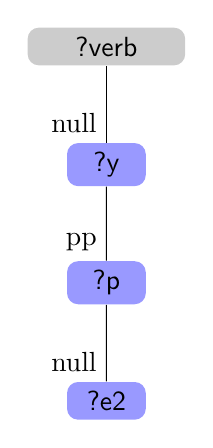
\begin{tikzpicture}
\node[fill = gray!40, shape = rectangle, rounded corners, minimum width = 2cm, font = \sffamily] (51) {?verb}
child {node[fill = blue!40, shape = rectangle, rounded corners, minimum width = 1cm, font = \sffamily]  (52) {?y}
child {node[fill = blue!40, shape = rectangle, rounded corners, minimum width = 1cm, font = \sffamily] (53) {?p}
child {node[fill = blue!40, shape = rectangle, rounded corners, minimum width = 1cm, font = \sffamily] (54) {?e2}
}
}};
\begin{scope}[nodes = {draw = none}]
\path (52)     -- (51) node [near start, left]  {\text{null}};
\path (53)     -- (52) node [near start, left]  {\text{pp}};
\path (54)     -- (53) node [near start, left]  {\text{null}};
\draw[densely dashed, rounded corners, thin];
\end{scope} 
\end{tikzpicture}
\caption{Visualisation for SPARQLPattern\_DE\_10}
\label{fig:SPARQLPatternDE10}
\end{figure}


\end{document}